%iffalse
\let\negmedspace\undefined
\let\negthickspace\undefined
\documentclass[journal,15pt,onecolumn]{IEEEtran}
\usepackage{cite}
\usepackage{amsmath,amssymb,amsfonts,amsthm}
\usepackage{algorithmic}

\usepackage{textcomp}
\usepackage[table,xcdraw]{xcolor}
\usepackage{txfonts}
\usepackage{listings}
\usepackage{enumitem}
\usepackage{mathtools}
\usepackage{gensymb}
\usepackage{enumitem}
\usepackage{comment}
\usepackage[breaklinks=true]{hyperref}
\usepackage{tkz-euclide} 
\usepackage{gvv}                                        
%\def\inputGnumericTable{}
\usepackage[latin1]{inputenc} 
\usepackage{xparse}
\usepackage{color}
\usepackage{graphicx}
\usepackage{array}                                            
\usepackage{longtable}                                       
\usepackage{calc}                                             
\usepackage{multirow}
\usepackage{multicol}
\usepackage{hhline}                                           
\usepackage{ifthen}                                           
\usepackage{lscape}
\usepackage{tabularx}
\usepackage{array}
\usepackage{float}
\newtheorem{theorem}{Theorem}[section]
\newtheorem{problem}{Problem}
\newtheorem{proposition}{Proposition}[section]
\newtheorem{lemma}{Lemma}[section]
\newtheorem{corollary}[theorem]{Corollary}
\newtheorem{example}{Example}[section]
\newtheorem{definition}[problem]{Definition}
\newcommand{\BEQA}{\begin{eqnarfnray}}
\newcommand{\EEQA}{\end{eqnarray}}
%\newcommand{\define}{\stackrel{\triangle}{=}}
\theoremstyle{remark}
%\newtheorem{rem}{Remark}
% Marks the beginning of the document

\begin{document}


\title{gate 1}
\author{AI25btech11037 - Stalin}
\maketitle
\renewcommand{\thefigure}{\theenumi}
\renewcommand{\thetable}{\theenumi}




\begin{enumerate}


  



\item 
When she fell down the \underline{\hspace{1cm}}, she received many \underline{\hspace{1cm}} but little help.

\vspace{0.5cm}

\hspace{1.3cm}The words that best fill the blanks in the above sentence are:\hfill \textbf{ (GATE AR 2018)}



\begin{enumerate}
\item   stairs, stares
\item  stairs, stairs 
\item  stares, stairs 
\item  stares, stares 
\end{enumerate}




\item 
In spite of being, he failed to correct his \underline{\hspace{2cm}} behaviour.\hfill \textbf{ (GATE AR 2018)}

 The word that best fills the blank in the above sentence is:
\begin{enumerate}
\item   rational 
\item   reasonable 
\item   errant 
\item   good 
\end{enumerate}


\vspace{01cm}


\item  For  $ 0 \leq x \leq 2\pi  $,  $ \sin x  $ and  $ \cos x  $ are both decreasing functions in the interval \underline{\hspace{1cm}}.\hfill \textbf{ (GATE AR 2018)}

\vspace{0.5cm}

\begin{enumerate} 
\item   $ \left( 0, \frac{\pi}{2} \right)  $
\item    $ \left( \frac{\pi}{2}, \pi \right)  $  
\item    $ \left( \pi, \frac{3\pi}{2} \right)  $  
\item    $ \left( \frac{3\pi}{2}, 2\pi \right)  $ 
\end{enumerate}

\vspace{0.8cm}

\item 
The area of an equilateral triangle is  $ \sqrt{3}  $. What is the perimeter of the triangle?\hfill \textbf{ (GATE AR 2018)}

\vspace{0.5cm}

\begin{enumerate}
\item  2 
\item  4 
\item  6 
\item  8 
\end{enumerate}

\vspace{0.5cm}


\item 
Arrange the following three-dimensional objects in the descending order of their volumes:\hfill \textbf{ (GATE AR 2018)}


\begin{enumerate}
    \item A cuboid with dimensions 10 cm, 8 cm and 6 cm
    \item A cube of side 8 cm
    \item A cylinder with base radius 7 cm and height 7 cm
    \item A sphere of radius 7 cm
\end{enumerate}



\begin{enumerate}
\item (i), (ii), (iii), (iv) 
\item (ii), (i), (iv), (iii) 
\item (iii), (ii), (i), (iv) 
\item (iv), (iii), (ii), (i) 
\end{enumerate}


\vspace*{1cm} % Add extra vertical space at the top

 \hspace{0.2cm} \textbf{Q.6 -- Q.10 carry two marks each.}


\item 
An automobile travels from city A to city B and returns to city A by the same route. The speed of the vehicle during the onward and return journeys were constant at 60 km/h and 90 km/h, respectively. What is the average speed in km/h for the entire journey? \hfill \textbf{ (GATE AR 2018)}



\begin{enumerate}

\item    72 
\item    73 
\item    74 
\item    75 

\end{enumerate}


\item  A set of 4 parallel lines intersect with another set of 5 parallel lines. How many parallelograms are formed?\hfill \textbf{ (GATE AR 2018)}

% Options
\vspace{0.5cm}

\begin{enumerate}
\item   20 
\item   48 
\item   60 
\item   72
\end{enumerate}


\item 
 To pass a test, a candidate needs to answer at least 2 out of 3 questions correctly. A total of 6,30,000 candidates appeared for the test. Question A was correctly answered by 3,30,000 candidates. Question B was answered correctly by 2,50,000 candidates. Question C was answered correctly by 2,60,000 candidates. Both questions A and B were answered correctly by 1,00,000 candidates. Both questions B and C were answered correctly by 90,000 candidates. Both questions A and C were answered correctly by 80,000 candidates. If the number of students answering all questions correctly is the same as the number answering none, how many candidates failed to clear the test?\hfill \textbf{ (GATE AR 2018)}
      

\begin{enumerate}
\item    30,000
 \item   2,70,000
 \item   3,90,000
 \item   4,20,000 
\end{enumerate}


 \item 
If $x^2 + x - 1 = 0$ what is the value of $x^4 + \dfrac{1}{x^4}$?\hfill \textbf{ (GATE AR 2018)}

\begin{enumerate}
    \item 1
    \item  5
    \item 7
    \item 9
\end{enumerate}


\item 
In a detailed study of annual crow births in India, it was found that there was relatively no growth during the period 2002 to 2004 and a sudden spike from 2004 to 2005. In another unrelated study, it was found that the revenue from cracker sales in India which remained fairly flat from 2002 to 2004, saw a sudden spike in 2005 before declining again in 2006. The solid line in the graph below refers to annual sale of crackers and the dashed line refers to the annual crow births in India. Choose the most appropriate inference from the above data.\hfill \textbf{ (GATE AR 2018)}

\begin{figure}[H]
    \centering
    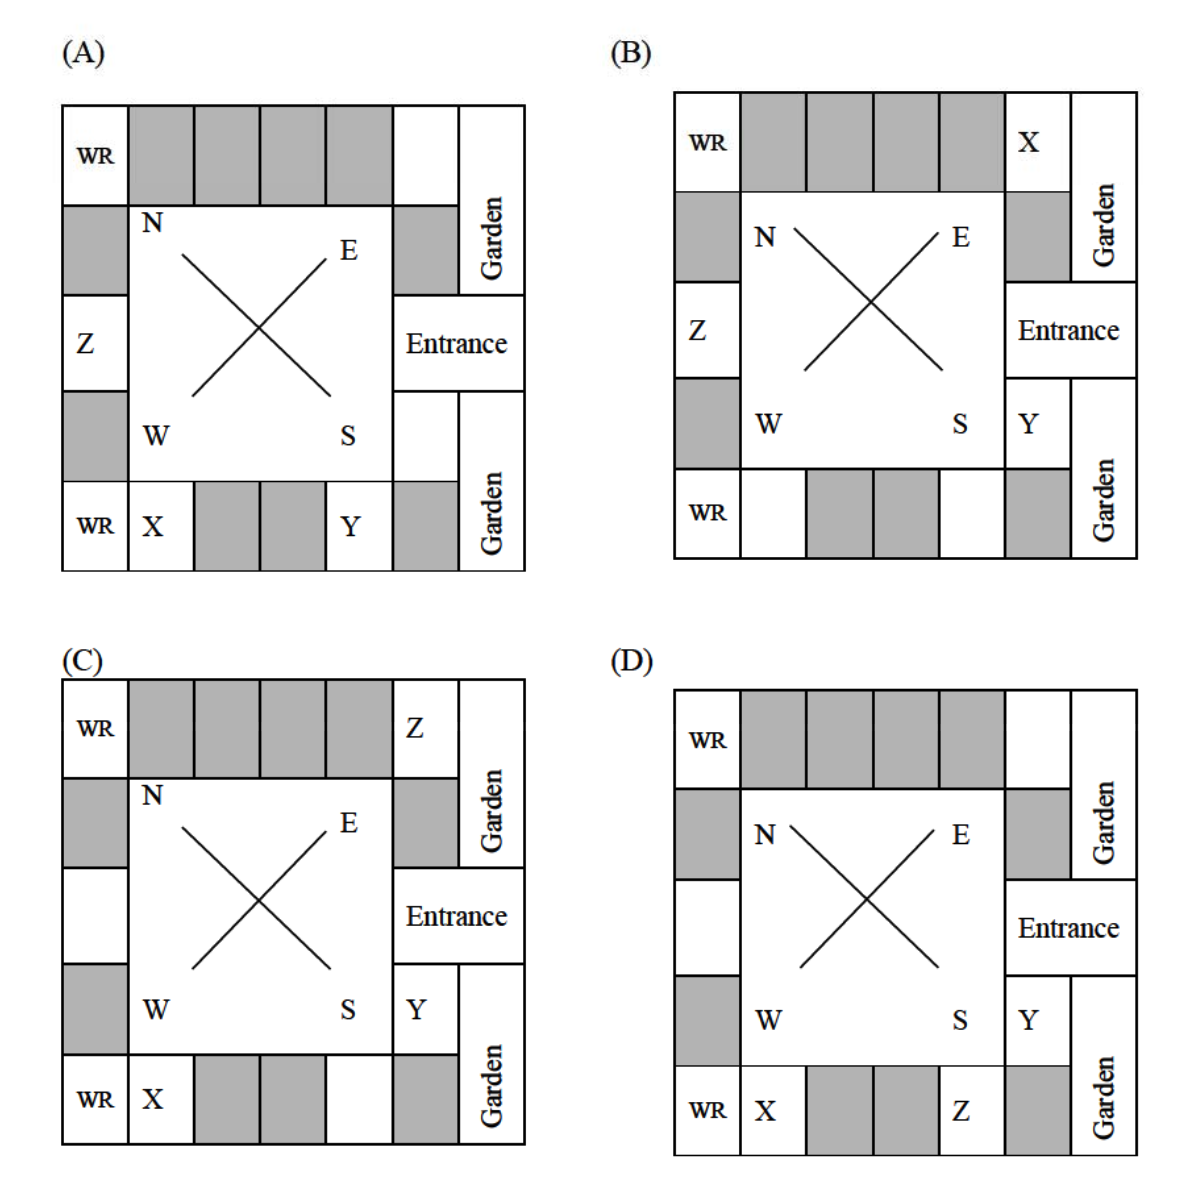
\includegraphics[width=0.5\linewidth]{figs/10i.png}
    \caption{}
    \label{fig:placeholder}
\end{figure}





\begin{enumerate}

\item    There is a strong correlation between crow birth and cracker sales.
\item   Cracker usage increases crow birth rate. 
\item    If cracker sale declines, crow birth will decline. 
\item   Increased birth rate of crows will cause an increase in the sale of crackers.
\end{enumerate}



\begin{center}
    \textbf{END OF THE QUESTION PAPER}
\end{center}


\vspace{0.6cm}
\textbf{Q.1--Q.25 carry one mark each.}

\vspace{0.5cm}
\item 
In a colour  Wheel, Red and Blues colours are \\\hfill \textbf{ (GATE AR 2018)}
 
\begin{enumerate}
\item    tertiary
\item    comblementary
\item    secondary
\item    primary
\end{enumerate} 


\item 
In a bird's eye perspective view of a cuboid, the maximum number of vanishing points is\hfill \textbf{ (GATE AR 2018)}

\vspace{0.5em}

\begin{enumerate}
\item    1 
\item    2
\item    3 
\item    6
\end{enumerate}

\vspace{1.5em}

\item 
The compressive strength of M-25 concrete is\hfill \textbf{ (GATE AR 2018)}

\vspace{0.5em}

\begin{enumerate}
\item  25 kg/sqm
\item  25 N/sqmm 
\item 250 N/sqmm 
\item 2.5 N/sqmm
\end{enumerate}

\vspace{1.5em}

\item 
In Critical Path Method (CPM) for time scheduling, 'forward pass calculation' is carried out for determining\hfill \textbf{ (GATE AR 2018)}

\vspace{0.5em}

\begin{enumerate}

\item  Late start and early finish time 
\item  Early start and early finish time 
\item  Late start and late finish time 
\item  Early start and late finish time
\end{enumerate}


\item 
Collapse of the World Trade Center (WTC), New York, in 2001, was due to\hfill \textbf{ (GATE AR 2018)}

\vspace{0.5em}

\begin{enumerate}
\item  Wind load failure 
\item  Foundation failure 
\item  Thermal performance failure of reinforcement steel in RCC
\item Thermal performance failure of structural steel
\end{enumerate}

\item 
During the construction of tall buildings, the equipment used for hoisting building materials to the upper floors is a\hfill \textbf{ (GATE AR 2018)}

\vspace{0.5em}

\begin{enumerate}
\item Goods lift
\item Capsule lift 
\item Gantry crane
\item  Tower crane
\end{enumerate}

\item 
A Rock-cut style of architecture is represented by\hfill \textbf{ (GATE AR 2018)}

\vspace{0.5em}
\begin{enumerate}
\item  Shyama Rama Temple, Bishnupur 
\item Kailasa Temple, Ellora 
\item Kandariya Mahadeva Temple, Khajuraho 
\item  Sanchi Stupa, Sanchi
\end{enumerate}

\vspace{1.5em}

\item 
'Area based development' and 'Pan city development' are part of\hfill \textbf{ (GATE AR 2018)}

\vspace{0.5em}

\begin{enumerate}
\item  Smart City Mission 
\item Digital India Mission 
\item Swachh Bharat Mission
\item Atal Innovation Mission
\end{enumerate}

\vspace{1cm}


\item 
In mass transportation, LRTS stands for\hfill \textbf{ (GATE AR 2018)}

\begin{flushleft}
\item    Light Rail Transit System\\
\item   Linear Rail Transit System\\
\item   Light Rail Transportation System\\
\item   Linear Rail Transportation System
\end{flushleft}


\vspace{0.5cm}

\item  The structural grid type shown in the figure below is a\hfill \textbf{ (GATE AR 2018)}


\begin{figure}[H]
    \centering
    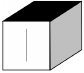
\includegraphics[width=0.25\linewidth]{figs/10.png}
 
\end{figure}



\begin{center}
\hspace{1cm}
  Tartan Grid \hspace{1cm}   Square Grid \hspace{1cm}   Rectangular Grid \hspace{1cm}   Irregular Grid
\end{center}

\vspace{0.4cm}

\noindent \textbf{Q.11} \hspace{0.5cm} Assuming other variables remaining constant, the Tropical Summer Index\hfill \textbf{ (GATE AR 2018)}
\vspace{0.05cm}


\begin{enumerate}

  \item  Increases with increase in air velocity 
  \item  Decreases with increase in wet-bulb temperature 
  \item  Decreases with increase in globe temperature 
  \item  Increases with increase in vapour pressure
\end{enumerate}

\vspace{0.15cm}

\item 
Government of India's urban development program 'HRIDAY' stands for\hfill \textbf{ (GATE AR 2018)}
\
\begin{enumerate}

    
  \item   Heritage Rejuvenation Implementation Development Aayog Yojana
  \item  Heritage Review Implementation Development Augmentation Yojana
  \item   Heritage City Development and Augmentation Yojana
  \item   Heritage City Improvement and Development Aawas Yojana
\end{enumerate}

\item 
As per the Urban and Regional Development Plan Formulation and Implementation (URDPFI) guidelines, the plan period considered in a 'Perspective plan' is\hfill \textbf{ (GATE AR 2018)}
\vspace{0.4cm}

\begin{enumerate}
    \item 1--10 years
    \item 11--15 years
    \item 20--30 years
    \item 35--45 years
\end{enumerate}

\item 
The Hall of Nations, New Delhi, was designed by\hfill \textbf{ (GATE AR 2018)}

\begin{enumerate}

    \item  Charles Correa
    \item  Raj Rewal 
    \item joseph Allen Stein
    \item  A. P. Kanvinde
\end{enumerate}
\vspace{0.6cm}

\item 
As per the National Building Code of India 2016, the minimum turning radius (in metres) required for fire tender movement is \hfill \textbf{ (GATE AR 2018)}


\begin{enumerate}
     \item   8.0 
     \item    8.5 
     \item   9.0 
     \item  9.6
     \end{enumerate}


 
\item 
Sidi Bashir Mosque with 'shaking Minarets' is located in\hfill \textbf{ (GATE AR 2018)}

\begin{enumerate}

\item   Ajmer 
\item  Allahabad 
\item   Ahmedabad
\item  Amritsar 
\end{enumerate}

\item 
Sight Distance' is considered in the degin of \hfill \textbf{ (GATE AR 2018)}


    
\begin{enumerate}
\item  Road intersection 
\item   Fenestration 
\item  Open kitchen 
\item   Auditorium 
\end{enumerate}

\vspace{0.5cm}

\textbf{Q.18} \hspace{0.3cm} In India, the term 'Town Planning Scheme' refers to\hfill \textbf{ (GATE AR 2018)}

\begin{enumerate}
\item   Land renewal 
\item   Land rejuvenation 
\item   Land reclamation
\item   Land readjustment 
\end{enumerate}

\vspace{0.5cm}

\textbf{Q.19} \hspace{0.3cm} Bamboo is a type of\hfill \textbf{ (GATE AR 2018)}


\begin{enumerate}
\item   Shrub 
\item    Timber 
\item   Evergreen tree 
\item    Perennial grass 
\end{enumerate}


\item 
According to the \textbf{UN}, one of the components for measuring 'inclusive growth' is\hfill \textbf{ (GATE AR 2018)}

\begin{enumerate}
    

\item   Economic well-being \item    Physical infrastructure 
\item   Education \item    Life expectancy 
\end{enumerate}



\item 
The unit of measurement of Damp Proof Course (DPC) in building construction is\hfill \textbf{ (GATE AR 2018)}

\begin{enumerate}
\item   kg \item    cum 
\item   sqm \item   rm 
\end{enumerate}



\item 
Which of the following is \textbf{NOT} a Building Information Modeling software tool\hfill \textbf{ (GATE AR 2018)}

\begin{enumerate}
\item   Adobe Illustrator \item     Bentley Microstation
    \item    Autodesk Revit  \item   Graphisoft ARCHICAD 
\end{enumerate}



\textbf{Q.23} \hspace{0.3cm} The concentric circles in a solar chart represent\hfill \textbf{ (GATE AR 2018)}\hfill

\begin{enumerate}
\item    Azimuth angle \item     Altitude angle 
 \item     Horizontal shadow angle \item    Vertical shadow angle 
\end{enumerate}

\item 
A room of 3m $\times$ 3m $\times$ 3m has a reverberation time of 0.8 sec. Using Sabin's method, the total absorption in the room is \rule{4cm}{0.15mm} sabin \textit{(up to one decimal place).} \hfill \textbf{ (GATE AR 2018)}

\vspace*{1cm} 

\item 
A 25 storeyed building has 5 lifts. The resulting waiting time is 35 sec and `Return Travel Time' is 175 sec. The number of lifts required for reducing waiting time to 25 sec, without increasing the lift speed, is \underline{\hspace{3cm}}.\hfill \textbf{ (GATE AR 2018)}
\vspace{1.5cm}

 

\item 
\textbf{Q.26 -- Q.55 carry two marks each.}
 Match the planning documents in \textbf{Group-I} with their respective government schemes in \textbf{Group-II} \hfill \textbf{ (GATE AR 2018)}

\vspace{0.5cm}

\hspace{2.5cm}\textbf{Group-I} \hspace{8cm} \textbf{Group-II} 

\begin{enumerate}
\item      Integrated Cluster Action Plan   \item  1  NULM 
\item      Service Level Improvement Plan   \item 2 Make in India
\item       Housing for All Plan of Action   \item  3  RuRBAN mission 
\item       City Livelihood Centre Development Plan   \item  4  PMAY                                                    \item 5  AMRUT 
\end{enumerate}
 
\begin{enumerate}
\item   P-4, Q-1, R-5, S-2  \item    P-3, Q-5, R-4, S-2 
\item    P-5, Q-1, R-4, S-3  \item    P-3, Q-5, R-4, S-1 
\end{enumerate}


\noindent \textbf{Q.27} \quad Associate the fire safety requirements for high rise buildings in \textbf{Group-I} with \\ \hfill \textbf{ (GATE AR 2018)}
\hspace*{3.3em} corresponding standards of the National Building Code of India 2016 in \textbf{Group-II} 


\textbf{Group-I} \hspace{8cm} \textbf{Group-II} 

\begin{enumerate}
\item      Minimum Refuge area                  \item   12.5 sqm/person
\item      Maximum Travel distance              \item  2.0 m 
\item      Maximum Occupant load                \item   0.3 sqm/person 
\item      Minimum Stair case width             \item 12.0 ton 
                                               \item  30.0 m 
\end{enumerate}

\bigskip

\begin{enumerate}
\item    P-4, Q-1, R-5, S-2 
\item   P-3, Q-5, R-4, S-1 
\item    P-3, Q-5, R-1, S-2 
\item    P-4, Q-5, R-1, S-3 
\end{enumerate}


 

 \item 
  Match the photometric quantities in \textbf{Group-I} with their respective units in \textbf{Group-II}\hfill \textbf{ (GATE AR 2018)}

 \textbf{Group-I}\hspace{8cm} \textbf{Group-II} \\
\vspace{0.15cm}
\begin{enumerate}
\item p  lluminance   \item  1   Candela 
\item  Q  uminous Intensity  \item  2  Candela/sqm 
\item  R  Luminance \item  3  Lumens/sqm
\item  S Luminous Efficacy  \item  4  Lumens/watt

                    \item  5  Lumens
\end{enumerate}

\vspace{0.5cm}





\begin{enumerate}

\item   P-3, Q-2, R-5, S-4 
\item   P-5, Q-4, R-2, S-1 
\item   P-5, Q-1, R-2, S-3
\item D) P-3, Q-1, R-2, S-4 
\end{enumerate}


\item 
Associate the symbols in \textbf{Group-I} with their meanings in \textbf{Group-II}




 
\vspace{0.15cm}

\textbf{Group-I}\hspace{8cm} \textbf{Group-II} 



\begin{figure} [h!]
    \centering
    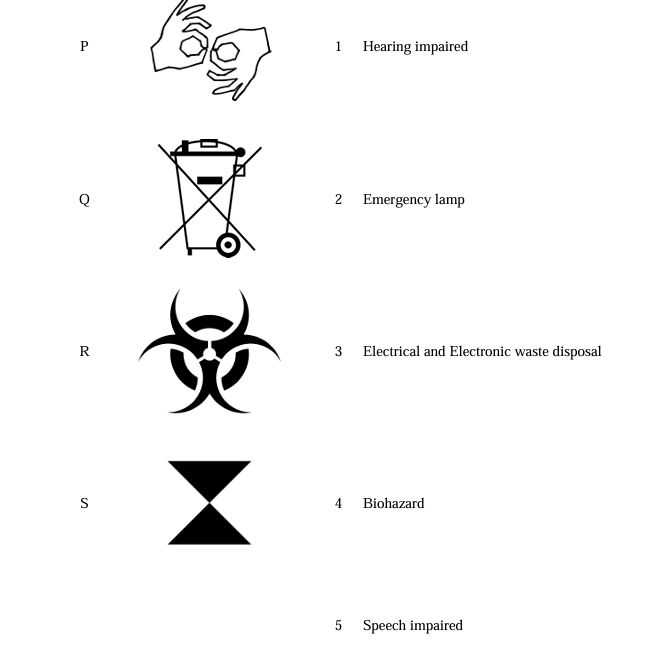
\includegraphics[width=1\linewidth]{figs/29.png}
  \end{figure}

 

\begin{multicols}{2}
\begin{enumerate}
\item P-5, Q-3, R-1, S-2
\item P-1, Q-5, R-3, S-4
\item P-1, Q-3, R-4, S-5
\end{enumerate}
\end{multicols}
\item 
Match the elements in \textbf{Group-I} with the building components in \textbf{Group-II}\hfill \textbf{ (GATE AR 2018)}

\vspace{0.15cm}

\textbf{Group-I}\hspace{8cm} \textbf{Group-II} 

\begin{enumerate}

\item  P  king post              \item  1 Curtain glazing 
\item  Q  beam                  \item  2  Door 
\item  R   Metal decking        \item 3 Plintch              
\item  S  jamb                  \item 4  intermidate field       
                               \item  5  Truss 
  
\end{enumerate}


\begin{enumerate}

\item    P-5, Q-3, R-4, S-1
\item    P-2, Q-4, R-3, S-1 
\item    P-2, Q-4, R-5, S-3 
\item    P-5, Q-3, R-4, S-2 

\end{enumerate}


\vspace{0.5cm}

\item 
Match the iconic architectural examples in \textbf{Group-I} with their predominant structural systems in \textbf{Group-II}\hfill \textbf{ (GATE AR 2018)}

\vspace{0.15cm}

\hspace{3cm}  \textbf{Group-I}\hspace{8cm} \textbf{Group-II} \\
\vspace{0.15cm}


\begin{enumerate}
    \item     \ Maria del Fiore Cathedral, Florence  \item   1. Shell
    \item    Notre Dame Cathedral, Paris  \item    2. Suspended roof
    \item     Notre Dame Cathedral, Paris  \item    3. Space frame
    \item    Baha'i Temple, Delhi 4. Double-walled dome \item    5. Flying buttress
\end{enumerate}

 
\begin{enumerate}
\item    P-5, Q-3, R-4, S-1
\item    P-2, Q-4, R-3, S-1 
\item    P-2, Q-4, R-5, S-3 
\item    P-5, Q-3, R-4, S-2 
\end{enumerate}


\vspace{0.5cm}

\item 
Match the building materials in \textbf{Group-I} with their distinctive properties in \textbf{Group-II}\hfill \textbf{ (GATE AR 2018)}

\vspace{4pt}

\vspace{4pt}

\hspace{3cm}  \textbf{Group-I}\hspace{8cm} \textbf{Group-II} 
\begin{enumerate}

\item     Cement    \item  1 Charring Charring
\item     steel     \item  2 Brittle
\item     wood      \item  3 Evaporation 
\item     glass     \item  4 Tensile strength 
                   \item  5  Setting Time   
\end{enumerate}

 
\begin{enumerate}
\item    P-5, Q-3, R-4, S-1
\item    P-2, Q-4, R-3, S-1
\item    P-2, Q-4, R-5, S-3 
\item    P-5, Q-3, R-4, S-2 
\end{enumerate}

\vspace{2cm}



\vspace{0.5cm}

\item 
Match the built forms in \textbf{Group-I} with their descriptions in \textbf{Group-II}\hfill \textbf{ (GATE AR 2018)}

\begin{multicols}{2}
\noindent \item  \textbf  {Group-I}
\begin{enumerate}
    \item     Agora
    \item     Ziggurat
    \item     Mastaba
    \item     Synagogue
\end{enumerate}

 \textbf{Group-II}
\begin{enumerate}
    \item Custodial precincts
    \item Place of Jewish worship
    \item Built in diminishing stages of masonry with buttressed wall
    \item Market place or public square
    \item Tomb made of mud bricks
\end{enumerate}
\end{multicols}


\begin{multicols}{2}
\begin{enumerate}
    \item P-1, Q-4, R-3, S-2
    \item P-4, Q-3, R-1, S-5
    \item P-4, Q-3, R-5, S-2
    \item P-3, Q-1, R-5, S-2
\end{enumerate}
\end{multicols}

% Q.34
\item 
Match the building configuration characteristics in \textbf{Group-I} with their seismic consequences in \textbf{Group-II}\hfill \textbf{ (GATE AR 2018)}

\begin{multicols}{2}
\noindent \hspace{2cm} \textbf  {Group-I}
\begin{enumerate}
    \item     Re-entrant corner
    \item     Floating column
    \item     Irregular storey stiffness
    \item     Gap between adjacent buildings
\end{enumerate}
 
\textbf{Group-II}
\begin{enumerate}
    \item Soft storey
    \item Stress concentration at corner
    \item Load path discontinuity
    \item Vertical asymmetry
    \item Pounding
\end{enumerate}
\end{multicols}

\begin{multicols}{2}
\begin{enumerate}
    \item P-3, Q-1, R-2, S-4
    \item P-2, Q-3, R-1, S-5
    \item P-4, Q-3, R-1, S-5
    \item P-3, Q-5, R-2, S-1
\end{enumerate}
\end{multicols}


\item 
Match the landscaping terms in \textbf{Group-I} with their descriptions in \textbf{Group-II}\hfill \textbf{ (GATE AR 2018)}

\begin{multicols}{2}
\noindent \item \textbf{Group-I}
\begin{enumerate}
    \item     Xeriscaping
    \item     Drip line
    \item     Swale
    \item     Turf block paver
\end{enumerate}

 \textbf{Group-II}
\begin{enumerate}
    \item Wide vegetated drain
    \item Tree rings
    \item Outermost circumference of a tree canopy
    \item Solution to topsoil erosion and water permeability
    \item A little or no irrigation
\end{enumerate}
\end{multicols}

\vspace{0.3cm}

\begin{multicols}{2}
\begin{enumerate}
    \item P-5, Q-3, R-1, S-4
    \item P-3, Q-5, R-1, S-4
    \item P-2, Q-3, R-1, S-5
    \item P-5, Q-2, R-4, S-1
\end{enumerate}
\end{multicols}


 

\item 
Match the planning principles in \textbf{Group-I} with their descriptions in \textbf{Group-II}\hfill \textbf{ (GATE AR 2018)}

 \begin{multicols}{2}
     
 
\hspace{1cm} \textbf{Group-I}
\begin{enumerate}
    \item     \hspace{0.2cm} Transit oriented development
    \item      \hspace{0.2cm} Core periphery theory
    \item      \hspace{0.2cm} Bid rent theory
    \item      \hspace{0.2cm} Cluster theory
\end{enumerate}


\textbf{Group-II}
\begin{enumerate}
    \item Four stage model of regional development
    \item Compact and walkable mixed use development
    \item Geographic concentration of inter-connected institutions
    \item Change of land price with relative distance from the CBD
    \item Interactive and participatory planning process
\end{enumerate}
\end{multicols}

\vspace{0.5cm}
\begin{multicols}{2}
    

\begin{enumerate}
    \item P-2, Q-1, R-4, S-3
    \item P-2, Q-1, R-5, S-3
    \item P-4, Q-2, R-5, S-3
    \item P-2, Q-3, R-5, S-4
\end{enumerate}
\end{multicols}
\vspace{0.5cm}

\item 
Match the cities in \textbf{Group-I} with their planners in \textbf{Group-II}\hfill \textbf{ (GATE AR 2018)}
\begin{multicols} {2}
 
 \textbf{Group-I}
\begin{enumerate}
    \item      \hspace{0.2cm} Islamabad
    \item      \hspace{0.2cm} Tel Aviv
    \item      \hspace{0.2cm} Bhubaneswar
    \item      \hspace{0.2cm} Brasilia
\end{enumerate}

\textbf{Group-II}
\begin{enumerate}
    \item Patrick Geddes
    \item C.A. Doxiadis
    \item Lucio Costa
    \item B. V. Doshi
    \item O. Koenigsberger
\end{enumerate}
\end{multicols}
\begin{multicols}{2}
\begin{enumerate}
    \item P-2, Q-4, R-1, S-3
    \item P-4, Q-1, R-5, S-2
    \item P-2, Q-1, R-5, S-3
    \item P-2, Q-3, R-4, S-5
\end{enumerate}
\end{multicols}


\item Match the Temples in \textbf{Group-I} with their Dynastic period in \textbf{Group-II}\hfill \textbf{ (GATE AR 2018)}
\begin{multicols}{2}
    

\textbf{Group-I}
\begin{enumerate}
    \item      \hspace{0.2cm} Brihadeshvara Temple
    \item      \hspace{0.2cm} Kailasanatha Temple
    \item      \hspace{0.2cm} Bhitargaon Temple
    \item      \hspace{0.2cm} Lad Khan Temple
\end{enumerate}
\columnbreak \noindent
\hspace{1cm} \textbf{Group-II}
\begin{enumerate}
    \item Gupta
    \item Chalukya
    \item Lodhi
    \item Chola
    \item Pallava
\end{enumerate}
\end{multicols}

\begin{multicols}{2}
\begin{enumerate}
    \item P-4, Q-5, R-1, S-2
    \item P-5, Q-1, R-2, S-3
    \item P-2, Q-5, R-1, S-3
    \item P-4, Q-1, R-2, S-5
\end{enumerate}
\end{multicols}



\item  Match the Buildings in \textbf{Group-I} with their Architects in \textbf{Group-II}\hfill \textbf{ (GATE AR 2018)}
\begin{multicols}{2}
    

\textbf{Group-I}
\begin{enumerate}
\item P Guggenheim Museum, Bilbao
\item Q The Shard, London
\item R Commerz Bank, Frankfurt
\item S Heydar Aliyev Centre, Baku
\end{enumerate}



\textbf{Group-II}
\begin{enumerate}
\item Richard Rogers
\item Norman Foster
\item Frank Gehry
\item Renzo Piano
\item Zaha Hadid
\end{enumerate}
\end{multicols}

\begin{multicols}{2}
\begin{enumerate}
\item P-3, Q-4, R-2, S-5
\item P-3, Q-4, R-1, S-2
\item P-2, Q-4, R-1, S-5
\item P-2, Q-5, R-4, S-3
\end{enumerate}
\end{multicols}

\vspace{1cm}


\item 
Match the following urban conservation themes in \textbf{Group-I} with their respective descriptions in \textbf{Group-II}\hfill \textbf{ (GATE AR 2018)}
\begin{multicols}{2}

\textbf{Group-I}
\begin{enumerate}
\item  Restoration
\item  Reconstitution
\item  Reconstruction
\item  Replication
\end{enumerate}

\textbf{Group-II}
\begin{enumerate}
\item Piece by piece re-assembly
\item Returning to previous stage
\item Physical addition
\item Re-creation of vanished elements
\item Reproduction of an exact copy
\end{enumerate}
\end{multicols}

\begin{multicols}{2}
\begin{enumerate}
\item P-2, Q-5, R-4, S-3
\item P-2, Q-1, R-4, S-5
\item P-3, Q-2, R-1, S-4
\item P-3, Q-1, R-3, S-5
\end{enumerate}
\end{multicols}

\vspace{1cm}

\item 
A Single Phase Neutral (SPN) electrical circuit has a power consumption of 330W. Considering a voltage of 110V and power factor of 0.8, the electrical current drawn is \underline{\hspace{3cm}} Amp \emph{(up to one decimal place)}.\hfill \textbf{ (GATE AR 2018)}

\vspace{1cm}

\item 
A building with 100 sqm roof area is connected to a 72 cum rainwater collection tank. If the rainfall is 60 mm per hour and the loss during water storage is 20\%, then the time taken to fill the tank completely is \underline{\hspace{3cm}} hours.\hfill \textbf{ (GATE AR 2018)}

 
\item 
The planning norms for provision of schools in a given town is shown below:\hfill \textbf{ (GATE AR 2018)}

\begin{table}[h!]
\centering
\begin{tabular}{|l|l|l|}
\hline
\textbf{Schools} & \textbf{Population norm} & \textbf{Land requirement per school} \\
\hline
Elementary School & One per 2500 persons & 0.4 hectare \\
Primary School    & One per 5000 persons & 1.0 hectare \\
Secondary School  & One per 12500 persons & 2.0 hectare \\
\hline
\end{tabular}
\end{table}

\item 

Total land area required for providing all types of schools for a population of 200,000 is \underline{\hspace{3cm}} hectares.


\item 
In a mixed use development on a 2.0 hectare site with 2.0 FAR, the ratio of residential to commercial floor area is 3:2. The minimum parking (in ECS) needed per 100 sqm of residential and commercial floor area is 1.0 and 1.25 respectively. Considering full FAR utilization, the total parking requirement is \underline{\hspace{3cm}} ECS.\hfill \textbf{ (GATE AR 2018)}


\item 
plotted housing scheme on a site of 12 hectare has 60\% saleable area. The average unit cost of land development is INR 300 million per hectare. If the profit margin is 20\%, then the selling price of land per hectare is \underline{\hspace{3cm}} million INR.\hfill \textbf{ (GATE AR 2018)}


\item  An isolated enclosure shown in the Figure has inlet \textbf{P} and outlet \textbf{Q} of 2 sqm each, on the opposite walls. The outdoor wind speed is 5 m/sec. If the coefficient of effectiveness is 0.6, the rate of natural ventilation in the enclosure (the required answer) is \underline{\hspace{3cm}}.\hfill \textbf{ (GATE AR 2018)}
\begin{figure} [h]
    \centering
    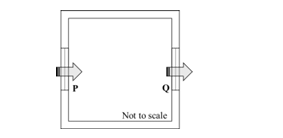
\includegraphics[width=0.3\linewidth]{figs/Screenshot 2025-08-16 142607.png}
    \caption{Caption}
    \label{fig:placeholder}
\end{figure}


\item 
A 5m $\times$ 5m $\times$ 3m room has four 230 mm thick external brick walls. Total wall fenestration is 10 sqm. The temperature difference between indoor and outdoor is 2 degC. The air to air transmittance values for 230 mm thick brick wall and 200 mm thick aerated concrete block wall are 2.4 and 1.7 W/sqm degC respectively. If the brick walls are replaced with the aerated concrete block walls, then the change in conductive heat flow through the walls is \underline{\hspace{3cm}} W.\hfill \textbf{ (GATE AR 2018)}

\item 
For an activity, 'optimistic time duration' is 4 days, 'pessimistic time duration' is 11 days and 'most-likely time duration' is 8 days. The PERT value of time duration is \underline{\hspace{2cm}} days \emph{(up to one decimal place)}.\hfill \textbf{ (GATE AR 2018)}

\begin{figure}[h]
    \centering
    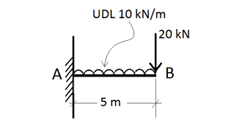
\includegraphics[width=0.4\linewidth]{figs/Screenshot 2025-08-16 133516.png}
    \caption{Caption}
    \label{fig:placeholder}
\end{figure}




\item 
The water consumption of a high rise apartment building with 60 dwelling units having an average household size of 5 persons is 135 lpcd. Assuming 80\% of the total use is met with recycled water supply, the daily domestic demand for the building is \underline{\hspace{3cm}} litres.\hfill \textbf{ (GATE AR 2018)}




\item 
In India, for 1.0 cum of M-20 grade concrete, the number of cement bags required is \underline{\hspace{3cm}} \emph{(up to two decimal places)}.\hfill \textbf{ (GATE AR 2018)}


\item 
The sound power level of an outdoor non-directional point source is 90 dB. Considering an atmospheric impedance of 400 rayls, the sound pressure level at 10 m distance from the source is \underline{\hspace{3cm}} dB.\hfill \textbf{ (GATE AR 2018)}


\item 
The live load and dead load in a three storeyed residential building, transferred through a single column, is 12 tons and 18 tons respectively. If the soil bearing capacity is 10 ton/sqm and the factor of safety is 1.5, the area of column footing is \underline{\hspace{3cm}} sqm \emph{(up to one decimal place)}.\hfill \textbf{ (GATE AR 2018)}


\item 
The indoor illumination requirement for a building is 350 Lux. If the daylight factor is 2.7 and the design sky illuminance is 9000 Lux, then the required supplementary artificial lighting is \underline{\hspace{3cm}} Lux.\hfill \textbf{ (GATE AR 2018)}


    \item 
    Two design options of a business building on a 10.0 hectare site are being compared for built up area. Floor to floor height of Option A is 3.6 m and that of Option B is 4.5 m. If the maximum allowable building height is 45 m with same ground coverage for both options, the additional built up area achievable in Option A over Option B is \underline{\hspace{3cm}} percent.
    \hfill \textbf{ (GATE AR 2018)}

\begin{center}
\textbf{END OF THE QUESTION PAPER}
\end{center}



\renewcommand{\arraystretch}{2.2} % row height
\setlength{\tabcolsep}{20pt} % column spacing
\item
\begin{tabular}{|c|c|c|c|c|}
\hline
\rowcolor{orange!30} % color for this row
\textbf{Q.No.} & \textbf{Type} & \textbf{Section} & \textbf{Key/Range} & \textbf{Marks} \\
\hline
1  & MCQ & GA & A & 1 \\ \hline
2  & MCQ & GA & C & 1 \\ \hline
3  & MCQ & GA & B & 1 \\ \hline
4  & MCQ & GA & C & 1 \\ \hline
5  & MCQ & GA & D & 1 \\ \hline
6  & MCQ & GA & A & 2 \\ \hline
7  & MCQ & GA & C & 2 \\ \hline
8  & MCQ & GA & D & 2 \\ \hline
9  & MCQ & GA & C & 2 \\ \hline
10 & MCQ & GA & A & 2 \\ \hline
1  & MCQ & AR & D & 1 \\ \hline
2  & MCQ & AR & C & 1 \\ \hline
3  & MCQ & AR & B & 1 \\ \hline
4  & MCQ & AR & B & 1 \\ \hline
5  & MCQ & AR & D & 1 \\ \hline
6  & MCQ & AR & D & 1 \\ \hline
7  & MCQ & AR & B & 1 \\ \hline
8  & MCQ & AR & A & 1 \\ \hline
9  & MCQ & AR & A & 1 \\ \hline
10 & MCQ & AR & A & 1 \\ \hline
11 & MCQ & AR & D & 1 \\ \hline
12 & MCQ & AR & C & 1 \\ \hline
13 & MCQ & AR & C & 1 \\ \hline
14 & MCQ & AR & B & 1 \\ \hline
15 & MCQ & AR & C & 1 \\ \hline
\end{tabular}
\vspace{1.5cm}


\renewcommand{\arraystretch}{2.2} % row height
\setlength{\tabcolsep}{20pt} % column spacing
\item
\begin{tabular}{|c|c|c|c|c|}
\hline
\rowcolor{orange!30}
Q.No. & Type & Section & Key/Range & Marks \\
\hline
16 & MCQ & AR & C & 1 \\
\hline
17 & MCQ & AR & A & 1 \\
\hline
18 & MCQ & AR & D & 1 \\
\hline
19 & MCQ & AR & D & 1 \\
\hline
20 & MCQ & AR & A (or) B (or) C & 1 \\
\hline
21 & MCQ & AR & C & 1 \\
\hline
22 & MCQ & AR & A & 1 \\
\hline
23 & MCQ & AR & B & 1 \\
\hline
24 & NAT & AR & 5.3 to 5.7 & 1 \\
\hline
25 & NAT & AR & 7.0 to 7.0 & 1 \\
\hline
26 & MCQ & AR & D & 2 \\
\hline
27 & MCQ & AR & C & 2 \\
\hline
28 & MCQ & AR & D & 2 \\
\hline
29 & MCQ & AR & D & 2 \\
\hline
30 & MCQ & AR & D & 2 \\
\hline
31 & MCQ & AR & C & 2 \\
\hline
32 & MCQ & AR & B & 2 \\
\hline
33 & MCQ & AR & C & 2 \\
\hline
34 & MCQ & AR & B & 2 \\
\hline
35 & MCQ & AR & A & 2 \\
\hline
36 & MCQ & AR & A & 2 \\
\hline
37 & MCQ & AR & C & 2 \\
\hline
38 & MCQ & AR & A & 2 \\
\hline
39 & MCQ & AR & D & 2 \\
\hline
40 & MCQ & AR & B & 2 \\
\hline
\end{tabular}



\renewcommand{\arraystretch}{2.2} % row height
\setlength{\tabcolsep}{20pt} % column spacing
\item
\begin{tabular}{|c|c|c|c|c|}
\hline
\rowcolor{orange!30}
Q.No. & Type & Section & Key/Range & Marks \\
\hline
41 & NAT & AR & 3.7 to 3.8 & 2 \\
\hline
42 & NAT & AR & 15.0 to 15.0 & 2 \\
\hline
43 & NAT & AR & 104 to 104 & 2 \\
\hline
44 & NAT & AR & 440 to 440 & 2 \\
\hline
45 & NAT & AR & 600 to 600 & 2 \\
\hline
46 & NAT & AR & 21600 to 21600 & 2 \\
\hline
47 & NAT & AR & 69.5 to 70.5 & 2 \\
\hline
48 & NAT & AR & 7.8 to 7.9 & 2 \\
\hline
49 & NAT & AR & 224 to 226 & 2 \\
\hline
50 & NAT & AR & 8100 to 8100 & 2 \\
\hline
51 & NAT & AR & 5 to 9 & 2 \\
\hline
52 & NAT & AR & 58 to 60 & 2 \\
\hline
53 & NAT & AR & 4.0 to 5.0 & 2 \\
\hline
54 & NAT & AR & 107 to 107 & 2 \\
\hline
55 & NAT & AR & 20 to 20 & 2 \\
\hline
\end{tabular}
\end{enumerate}
\end{document}